\chapter{Time reasoning}


\section{Propositional logic}

\begin{description}
    \item[State] \marginnote{State} 
        The current state of the world can be represented as a set of propositions that are true according to the observation of an agent.

        The union of a countable sequence of states represents the evolution of the world. Each proposition is distinguished by its time step.

        \begin{example}
            A child has a bow and an arrow and then shoots the arrow.
            \[
                \begin{split}
                    \text{KB}^0 &= \{ \texttt{hasBow}^0, \texttt{hasArrow}^0  \} \\
                    \text{KB}^1 &= \{ \texttt{hasBow}^0, \texttt{hasArrow}^0, \texttt{hasBow}^1, \lnot\texttt{hasArrow}^1  \} 
                \end{split}
            \]
        \end{example}

    \item[Action] \marginnote{Action}
        An action indicates how a state evolves into the next one.
        It is described using effect axioms in the form:
        \[ \texttt{action}^t \Rightarrow (\texttt{preconditions}^t \iff \texttt{effects}^{t+1}) \]

        \begin{description}
            \item[Frame problem] \marginnote{Frame problem}
                The effect axioms of an action do not tell what remains unchanged in the next state.

            \begin{description}
                \item[Frame axioms] \marginnote{Frame axioms}
                    The frame axioms of an action describe the unaffected propositions of an action.
            \end{description}
        \end{description}

        \begin{example}
            The action of shooting an arrow can be described as:
            \[
                \begin{split}
                    \texttt{SHOOT}^t &\Rightarrow \{ \texttt{hasArrow}^t \iff \lnot\texttt{hasArrow}^{t+1} \} \\
                    \texttt{SHOOT}^t &\Rightarrow \{ \texttt{hasBow}^t \iff \texttt{hasBow}^{t+1} \}
                \end{split}  
            \]
        \end{example}

        Note that with $m$ actions and $n$ propositions, the number of frame axioms will be of order $O(mn)$.
        Inference for $t$ time steps will have complexity $O(nt)$.
\end{description}



\section{Situation calculus (Green's formulation)}
Situation calculus uses first-order logic instead of propositional logic.

\begin{description}
    \item[Situation] \marginnote{Situation}
        The initial state is a situation.
        Applying an action in a situation is a situation:
        \[ s \text{ is a situation and } \texttt{a} \text{ is an action} \iff \texttt{result}(\texttt{a}, s) \text{ is situation} \]
        (Note: in FAIRK module 1, \texttt{result} is denoted as \texttt{do}).

    \item[Fluent] \marginnote{Fluent}
        Function that varies depending on the situation 
        (i.e. tells if a property holds in a given situation).

        \begin{example}
            $\texttt{hasBow}(s)$ where $s$ is a situation.
        \end{example}

    \item[Action] \marginnote{Action}
        Actions are described using:
        \begin{descriptionlist}
            \item[Possibility axioms] \marginnote{Possibility axioms}
                Indicates the preconditions $\phi_\texttt{a}$ of an action \texttt{a} in a given situation $s$:
                \[ \phi_\texttt{a}(s) \Rightarrow \texttt{poss}(\texttt{a}, s) \]

            \item[Successor state axiom] \marginnote{Successor state axiom}
                The evolution of a fluent $F$ follows the axiom:
                \[ F^{t+1} \iff (\texttt{ActionCauses$(F)$} \vee (F^{t} \land \lnot\texttt{ActionCauses$(\lnot F)$})) \]
                In other words, a fluent is true if an action makes it true or does not change if the action does not involve it.

                Adding the notion of possibility, an action can be described as:
                \[ 
                    \begin{split}
                        \texttt{poss}&(\texttt{a}, s) \Rightarrow \Big( F(\texttt{result}(\texttt{a}, s)) \iff \\
                            & (\texttt{a} = \texttt{ActionCauses$(F)$}) \,\vee\, \\
                            & (F(s) \,\land\, \texttt{a} \neq \lnot\texttt{ActionCauses$(\lnot F)$})
                        \Big)
                    \end{split}
                \]
            
            \item[Unique action axiom] \marginnote{Unique action axiom}
                Only a single action can be executed in a situation to avoid non-determinism.
        \end{descriptionlist}
\end{description}



\section{Event calculus (Kowalski's formulation)}

Event calculus reifies fluents and events (actions) as terms (instead of predicates).

\begin{description}
    \item[Event calculus ontology] \marginnote{Event calculus ontology}
        A fixed set of predicates:
        \begin{descriptionlist}
            \item[$\texttt{holdsAt}(F, T)$] The fluent $F$ holds at time $T$.
            \item[$\texttt{happens}(\texttt{E}, T)$] The event \texttt{E} (i.e. execution of an action) happened at time $T$.
            \item[$\texttt{initiates}(\texttt{E}, F, T)$] The event \texttt{E} causes the fluent $F$ to start holding at time $T$.
            \item[$\texttt{terminates}(\texttt{E}, F, T)$] The event \texttt{E} causes the fluent $F$ to cease holding at time $T$.
            \item[$\texttt{clipped}(T_i, F, T_j)$] The fluent $F$ has been made false between the times $T_i$ and $T_j$ ($T_i < T_j$).
            \item[$\texttt{initially}(F)$] The fluent $F$ holds at time 0.
        \end{descriptionlist}

    \item[Domain-independent axioms] \marginnote{Domain-independent axioms}
        A fixed set of axioms:
        \begin{description}
            \item[Truthness of a fluent] \phantom{}
                \begin{enumerate}
                    \item A fluent holds if an event initiated it in the past and has not been clipped.
                        \[ 
                            \begin{split}
                                \texttt{holdsAt}(F, T_j) \Leftarrow\, &\texttt{happens}(\texttt{E}, T_i) \land (T_i < T_j) \,\land\\
                                    &\texttt{initiates}(\texttt{E}, F, T_i) \land \lnot\texttt{clipped}(T_i, F, T_j)
                            \end{split}
                        \]

                    \item A fluent holds if it was initially true and has not been clipped.
                        \[ \texttt{holdsAt}(F, T) \Leftarrow\, \texttt{initially}(F) \land \lnot\texttt{clipped}(0, F, T) \]
                \end{enumerate}
                Note: the negations make the definition of these axioms in Prolog unsafe.
            
            \item[Clipping of a fluent]
                \[ \texttt{clipped}(T_i, F, T_j) \Leftarrow \texttt{happens}(\texttt{E}, T) \land (T_i < T < T_j) \land \texttt{terminates}(\texttt{E}, F, T) \]
        \end{description}

    \item[Domain-dependent axioms] \marginnote{Domain-dependent axioms}
        Domain-specific axioms defined using the predicates\\\texttt{initially}, \texttt{initiates} and \texttt{terminates}.
\end{description}

\begin{description}
    \item[Deductive reasoning] 
        Event calculus only allows deductive reasoning: 
        it takes as input the domain-dependant axioms and a set of events and computes a set of true fluents.
        If a new event is observed, the query needs to be recomputed again.
\end{description}


\begin{example}
    A room with a light and a button can be described as:
    \begin{descriptionlist}
        \item[Fluents] \texttt{lightOn} $\cdot$ \texttt{lightOff}
        \item[Events] \texttt{PUSH\_BUTTON}
    \end{descriptionlist}

    Domain-dependent axioms are:
    \begin{descriptionlist}
        \item[Initial state] \texttt{initially}(\texttt{lightOff}) 
        \item[Effects of \texttt{PUSH\_BUTTON} on \texttt{lightOn}] \phantom{}
            \begin{itemize}
                \item $\texttt{initiates}(\texttt{PUSH\_BUTTON}, \texttt{lightOn}, T) \Leftarrow \texttt{holdsAt}(\texttt{lightOff}, T)$
                \item $\texttt{terminates}(\texttt{PUSH\_BUTTON}, \texttt{lightOn}, T) \Leftarrow \texttt{holdsAt}(\texttt{lightOn}, T)$
            \end{itemize}
        \item[Effects of \texttt{PUSH\_BUTTON} on \texttt{lightOff}] \phantom{}
            \begin{itemize}
                \item $\texttt{initiates}(\texttt{PUSH\_BUTTON}, \texttt{lightOff}, T) \Leftarrow \texttt{holdsAt}(\texttt{lightOn}, T)$
                \item $\texttt{terminates}(\texttt{PUSH\_BUTTON}, \texttt{lightOff}, T) \Leftarrow \texttt{holdsAt}(\texttt{lightOff}, T)$
            \end{itemize}
    \end{descriptionlist}

    A set of events could be:
    \[ \texttt{happens}(\texttt{PUSH\_BUTTON}, 3) \cdot \texttt{happens}(\texttt{PUSH\_BUTTON}, 5) \cdot \texttt{happens}(\texttt{PUSH\_BUTTON}, 6) \]
\end{example}


\subsection{Reactive event calculus}
\marginnote{Reactive event calculus}

Allows to add events dynamically without the need to recompute the result.



\section{Allen's logic of intervals}

Event calculus only captures instantaneous events that happen at given points in time.

\begin{description}
    \item[Allen's logic of intervals] \marginnote{Allen's logic of intervals}
        Reasoning on time intervals.

        \begin{description}
            \item[Interval] \marginnote{Interval} 
                An interval $i$ starts at a time $\texttt{begin}(i)$ and ends at a time $\texttt{end}(i)$.

            \item[Temporal operators] \marginnote{Temporal operators}
                \begin{itemize}
                    \item $\texttt{meet}(i, j) \iff \texttt{end}(i) = \texttt{begin}(j)$
                    \item $\texttt{before}(i, j) \iff \texttt{end}(i) < \texttt{begin}(j)$
                    \item $\texttt{after}(i, j) \iff \texttt{before}(j, i)$
                    \item $\texttt{during}(i, j) \iff \texttt{begin}(j) < \texttt{begin}(i) < \texttt{end}(i) < \texttt{end}(j)$
                    \item $\texttt{overlap}(i, j) \iff \texttt{begin}(i) < \texttt{begin}(j) < \texttt{end}(i) < \texttt{end}(j)$
                    \item $\texttt{starts}(i, j) \iff \texttt{begin}(i) = \texttt{begin}(j)$
                    \item $\texttt{finishes}(i, j) \iff \texttt{end}(i) = \texttt{end}(j)$
                    \item $\texttt{equals}(i, j) \iff \texttt{starts}(i, j) \land \texttt{ends}(i, j)$
                \end{itemize}

                \begin{figure}[H]
                    \centering
                    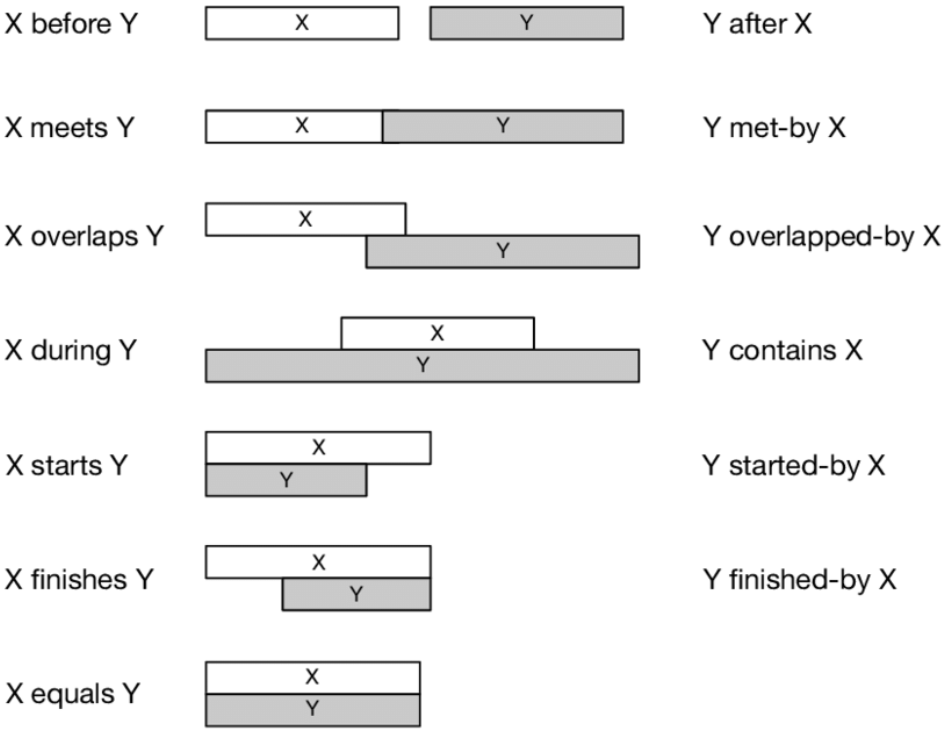
\includegraphics[width=0.5\textwidth]{img/allen_intervals.png}
                    \caption{Visual representation of temporal operators}
                \end{figure}
        \end{description}
\end{description}



\section{Modal logics}

Logic-based on interacting agents with their own knowledge base.

\begin{description}
    \item[Propositional attitudes] \marginnote{Propositional attitudes}
        Operators to represent knowledge and beliefs of an agent towards the environment and other agents.

        First-order logic is not suited to represent these operators.

    \item[Modal logics] \marginnote{Modal logics}
        Modal logics have the same syntax as first-order logic with the addition of modal operators.

    \item[Modal operator]
        A modal operator takes as input the name of an agent and a sentence (instead of a term as in FOL).
        
        \begin{description}
            \item[Knowledge operator] \marginnote{Knowledge operator}
                Operator to indicate that an agent \texttt{a} knows $P$:
                \[ \textbf{K}_\texttt{a}(P) \]

            \item[Belief operator]
            \item[Everyone knows operator]
            \item[Common knowledge operator]
            \item[Distribute knowledge operator]
        \end{description}

        Depending on the operators, different modal logics can be defined.

    \item[Semantics]
        An agent has a current perception of the world and considers the unknown as other possible worlds.
        Moreover, if $P$ is true in any accessible world from the current one, the agent has knowledge of $P$.

        Formally, semantics is defined on a set of primitive propositions $\phi$ 
        using a Kripke structure $M = (S, \pi, K_\texttt{1}, \dots, K_\texttt{n})$ where:
        \begin{itemize}
            \item $S$ is a set of states of the world.
            \item $\pi: \phi \rightarrow 2^S$ specifies in which states each primitive proposition holds.
            \item $K_\texttt{i} \subseteq S \times S$ is a binary relation where 
                $(s, t) \in K_\texttt{i}$ if an agent \texttt{i} considers the world $t$ possible (accessible) from $s$.
                In other words, when the agent is in the world $s$, it considers $t$ to be a possibly valid world.
                Obviously, $(s, s) \in K_\texttt{i}$ for all states.
        \end{itemize}

        \begin{example}
            Alice is in a room and tosses a coin. Bob is in another room and will enter Alice's room when the coin lands to observe the result.

            We define a model $M = (S, \pi, K_\texttt{a}, K_\texttt{b})$ on $\phi$ where:
            \begin{itemize}
                \item $\phi = \{ \texttt{tossed}, \texttt{heads}, \texttt{tails} \}$.
                \item $S = \{ s_0, h_1, t_1, h_2, t_2 \}$ where the possible states are divided in three stages:
                    the initial state ($s_0$), the result of the coin flip ($h_1, t_1$) and the observation of Bob ($h_2, t_2$).
                \item 
                    $\pi(\texttt{tossed}) = \{ h_1, t_1, h_2, t_2 \}$\\
                    $\pi(\texttt{heads}) = \{ h_1, h_2 \}$\\
                    $\pi(\texttt{tails}) = \{ t_1, t_2 \}$
                \item 
                    $K_\texttt{a} = \{ (s, s) \mid s \in S \}$ as Alice observes everything in each world and does not have doubts.\\
                    $K_\texttt{b} = \{ (s, s) \mid s \in S \} \cup \{ (h_1, t_1), (t_1, h_1) \}$ as Bob is unsure of what happens in the second stage.\\
            \end{itemize}
            \vspace*{-1em}
            With this model, we can determine the truthness of sentences like:
            \[ (M, s_0) \models K_\texttt{a}(\lnot\texttt{tossed}) \land K_\texttt{b}\Big(K_\texttt{a}\big(K_\texttt{b}(\lnot \texttt{heads} \land \lnot \texttt{tails})\big)\Big) \]
            \[ (M, t_1) \models (\texttt{heads} \vee \texttt{tails}) \land \lnot\texttt{K}_\texttt{b}(\texttt{heads}) \land 
                \lnot\texttt{K}_\texttt{b}(\texttt{tails}) \land 
                \texttt{K}_\texttt{b}(\texttt{K}_\texttt{a}(\texttt{heads}) \vee \texttt{K}_\texttt{a}(\texttt{tails})) \]
        \end{example}
    
    \item[Axioms] \phantom{}
        \begin{description}
            \item[Tautology] 
                All propositional tautologies are valid.

            \item[Modus ponens] 
                If $\varphi$ and $\varphi \Rightarrow \psi$ are valid, then $\psi$ is valid.

            \item[Distribution axiom] 
                Knowledge is closed under implication:
                \[ (K_\texttt{i}(\varphi) \land K_\texttt{i}(\varphi \Rightarrow \psi)) \Rightarrow K_\texttt{i}(\psi) \]

            \item[Knowledge generalization rule] 
                An agent knows all the tautologies:
                \[ \forall \text{ structures } M: (M \models \varphi) \Rightarrow (M \models K_\texttt{i}(\varphi)) \]

            \item[Knowledge axiom] 
                If an agent knows $\varphi$, then $\varphi$ is true:
                \[ K_\texttt{i}(\varphi) \Rightarrow \varphi \]

                In belief logic, this axiom is substituted with $\lnot K_\texttt{i}(\texttt{false})$.

            \item[Introspection axioms]
                An agent is sure of its knowledge:
                \begin{description}
                    \item[Positive] $K_\texttt{i}(\varphi) \Rightarrow K_\texttt{i}(K_\texttt{i}(\varphi))$ 
                    \item[Negative] $\lnot K_\texttt{i}(\varphi) \Rightarrow K_\texttt{i}(\lnot K_\texttt{i}(\varphi))$ 
                \end{description}
        \end{description}
        
        Different modal logics can be defined based on the valid axioms.
\end{description}



\section{Temporal logics}

Logics based on modal logic with the addition of a temporal dimension.
Time is discrete and each world is labeled with an integer. 
The accessibility relation maps into the temporal dimension with two possible evolution alternatives:
\begin{descriptionlist}
    \item[Linear-time] \marginnote{Linear-time}
        From each world, there is only one other accessible world.
    
    \item[Branching-time] \marginnote{Branching-time}
        From each world, there are many accessible worlds.
\end{descriptionlist}




\subsection{Linear-time temporal logic}

\begin{description}
    \item[Operators] \phantom{}
        \begin{description}
            \item[Next ($\bigcirc \varphi$)] \marginnote{Next}
                $\varphi$ is true in the next time step.

            \item[Globally ($\square \varphi$)] \marginnote{Globally}
                $\varphi$ is always true from now on.

            \item[Future ($\diamond \varphi$)] \marginnote{Future}
                $\varphi$ is true sometimes in the future.
                It is equivalent to $\lnot\square(\lnot \varphi)$.

            \item[Until ($\varphi \mathcal{U} \psi$)] \marginnote{Until}
                There exists a moment (now or in the future) when $\psi$ holds. 
                $\varphi$ is guaranteed to hold from now until $\psi$ starts to hold.

            \item[Weak until ($\varphi \mathcal{W} \psi$)] \marginnote{Weak until}
                There might be a moment when $\psi$ holds. 
                $\varphi$ is guaranteed to hold from now until $\psi$ possibly starts to hold.
        \end{description}

    \item[Semantics]
        Given a Kripke structure, $M = (S, \pi, K_\texttt{1}, \dots, K_\texttt{n})$ where states are represented using integers,
        the semantic of the operators is the following:
        \begin{itemize}
            \item $(M, i) \models P \iff i \in \pi(P)$.
            \item $(M, i) \models \bigcirc\varphi \iff (M, i+1) \models \varphi$.
            \item $(M, i) \models \square\varphi \iff \forall j \geq i: (M, j) \models \varphi$.
            \item $(M, i) \models \varphi \mathcal{U} \psi \iff \exists k \geq i: \big( (M, k) \models \psi \,\land\, \forall j. i \leq j \leq k: (M, j) \models \varphi \big)$.
            \item $(M, i) \models \varphi \mathcal{W} \psi \iff ((M, i) \models \varphi \mathcal{U} \psi) \vee ((M, i) \models \square\varphi)$.
        \end{itemize}

    \item[Model checking] \marginnote{Model checking}
        Methods to prove properties of linear-time temporal logic-based finite state machines or distributed systems.
\end{description}